\documentclass{article}

\usepackage[top=3cm, bottom=3cm, left=3cm, right=3cm]{geometry} % Page
\usepackage[utf8]{inputenc} % Encoding

\usepackage{graphicx}       % Images
\usepackage{paralist}       % Lists
\usepackage{float}          % In place images
\usepackage{color}          % Define colors
\usepackage[table]{xcolor}  % Colorize tables
\usepackage{chngpage}       % Redefine margins
\usepackage{multicol}       % Multiple columns

\addtolength{\parskip}{\baselineskip}    % Paragraph spacing
\linespread{1.15}                        % Lines spacing
\setlength{\plitemsep}{0.5\baselineskip} % List items spacing

% Colors
\definecolor{deepred}{RGB}{150,0,0}
\definecolor{deepgreen}{RGB}{0,150,0}
\definecolor{deepblue}{RGB}{0,0,70}
\definecolor{gray97}{gray}{.97}
\definecolor{gray90}{gray}{.90}
\definecolor{gray85}{gray}{.85}
\definecolor{gray75}{gray}{.75}
\definecolor{gray45}{gray}{.45}

% Remove numbering on sections
\setcounter{secnumdepth}{0}

% Helpers
\newcommand{\superscript}[1]{\ensuremath{^{\textrm{\small#1}}}}
\newcommand{\subscript}[1]{\ensuremath{_{\textrm{\small#1}}}}
\newcommand{\HRule}{\noindent\rule{\linewidth}{0.5mm}}

% Heading definitions
\makeatletter
\renewcommand\section{\@startsection
  {section}{1}{0mm}%                 name, level, indent
  {0cm}%                             beforeskip
  {0.01cm}%                          afterskip
  {\Huge\bfseries\color{black}}}%    style
\makeatother

% Links
\usepackage[urlcolor=blue,colorlinks=true,hyperfootnotes=false]{hyperref}
\hypersetup{linkcolor=deepblue,}

\begin{document}

\HRule

\section{Optimal Binary Search Trees}

\noindent{\huge Dynamic programming.} \\[0.4cm]
{\LARGE Operation Research.}\\[0.4cm]
\HRule \\[0.5cm]
\indent The goal of the maximum weight independent set problem (MWIS) is to compute, for a given set of geometric objects with certain weights, a subset of disjoint (non-overlapping) objects with maximum total weight.

There is a PTAS (polynomial-time algorihtm scheme) for MWIS in disk graphs, provided that a disk representation of the graph is given. 
The running-time for achieving approximation ratio $1+\epsilon$ 
is $n^{O(1/\epsilon^{2})}$ for a disk graph with n disks.\\[0.5cm]
\noindent{\Large Details:}
\begin{compactitem}
\item Executed on : \textsc{Ter Out 07 09:26:48 BRT 2014}. 
\item Number of disks : \textsc{1}. 
\item Execution time : \textsc{1,132668 seconds}. 
\item Memory required : \textsc{172 bytes}. 
\end{compactitem}

\subsection{Nodes}
\begin{table}[!ht]
\centering
\begin{tabular}{c||c|c|}
\cline{2-3}
 & \cellcolor{gray90}\textbf{Name} & \cellcolor{gray90}\textbf{Probabilities}  \\
\hline\hline
\multicolumn{1}{|c||}{\cellcolor{gray90}\textbf{1}} & A0 & 0,00 \\ \hline
\end{tabular}
\caption{Nodes probabilities.}
\end{table}

\newpage
\newpage
\tableofcontents
\newpage

\subsection{Execution}
\begin{table}[!ht]
\begin{adjustwidth}{-3cm}{-3cm}
\centering
\begin{tabular}{c||c|c|}
\cline{2-3}
 & \cellcolor{gray90}\textbf{1} & \cellcolor{gray90}\textbf{2} \\
\hline\hline
\multicolumn{1}{|c||}{\cellcolor{gray90}\textbf{0}} & 0,00 & 340282346638528859811704183484516925440,00 \\ \hline
\multicolumn{1}{|c||}{\cellcolor{gray90}\textbf{1}} &  & 0,00 \\ \hline
\end{tabular}
\caption{Table A.}
\end{adjustwidth}
\end{table}

\begin{table}[!ht]
\begin{adjustwidth}{-3cm}{-3cm}
\centering
\begin{tabular}{c||c|c|}
\cline{2-3}
 & \cellcolor{gray90}\textbf{1} & \cellcolor{gray90}\textbf{2} \\
\hline\hline
\multicolumn{1}{|c||}{\cellcolor{gray90}\textbf{0}} & 0 & 0 \\ \hline
\multicolumn{1}{|c||}{\cellcolor{gray90}\textbf{1}} &  & 0 \\ \hline
\end{tabular}
\caption{Table R.}
\end{adjustwidth}
\end{table}


\subsection{Analisis}
\begin{figure}[H]\centering
\noindent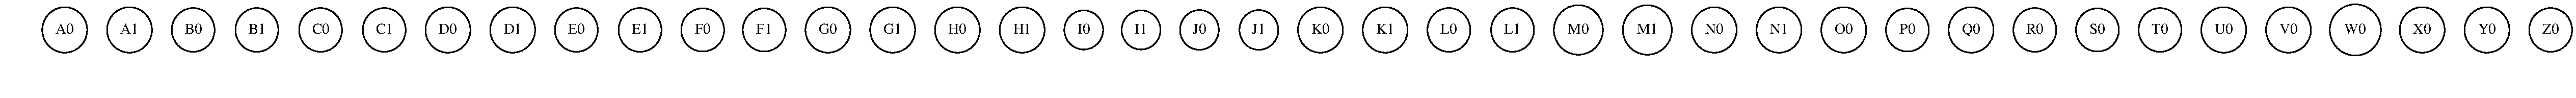
\includegraphics[height=500px, width=400px, keepaspectratio]{reports/tree.pdf}
\caption{Optimal search tree.}
\end{figure}
\newpage

\subsection{Digest}
\begin{compactitem}
\item Total nodes : {\Large 1}.
\item Levels : {\Large 1}.
\item Expected cost : {\Large 340282346638528859811704183484516925440,00}.
\end{compactitem}

\end{document}

